% TODO: Maybe rename "Manually Developed Algorithm"

\section{Search Algorithms}
This section describes the development of distributed algorithms that enable a group of robots to search a map for an object. These algorithms are implemented in the \texttt{botbrain} library. \\

This project explores two approaches for controlling the behavior of the robot swarm: manually developed algorithms and an algorithm based on reinforcement learning. The following sections describe the development of these approaches.

\subsection{Target Contributions}
A robot keeps track of its state which, together with sensor inputs, dictates how it moves and explores the environment. Different inputs may indicate that the robot should take different actions at the same time. For example, the robot may {\color{red} know} that an unexplored area exists in front of it, but it is blocked by an obstacle. The exploration part of the behavior may tell the robot to move towards the unexplored area, while the obstacle avoidance part may {\color{red} tell} the robot to move away from the obstacle. These subsystems should all contribute to the behavior of the robot at the same time. To resolve this, each subsystem outputs a "target" vector, which signifies the direction the robot should move. The target vectors are summed to get a single target vector which specifies the direction that the robot should move. Each subsystem can be weighted to make the robot more responsive to that subsystem. The obstacle avoidance subsystem should, for example, be weighted highly, as the robot should avoid the robot hitting obstacles. \Cref{fig:target-contributions} shows an illustration of this procedure.

\begin{figure}[H]
    \begin{center}
        \includegraphics[width=0.75\textwidth]{figures/target-contribtions.png}
    \end{center}
    \caption{Example of the target calculation}
    \label{fig:target-contributions}
\end{figure}


% TODO: Describe the idea, that different factors contribute to the target vector. The target vector is the sum over all contributions.
% TODO: Describe how we take gradients on a grid

\subsection{Search Grid}

Each robot has a "search grid" which is continuously updated by observations from the robot itself, and the observations of other robots which it receives over the shared communication channel. The "search grid" can be thought of as a heat map, where well-explored areas are "colder" and less explored areas are "hotter". If communication between robots is lossless, the internal "search grids" of all robots should always be in sync. Each robot will then calculate its desired trajectory vector by taking a gradient over the "search grid" at its current position (see \cref{fig:search-gradient}). This results in behavior where robots will seek out unexplored areas near them. \\
\begin{figure}[h]
    \begin{center}
        % TODO: Actually create figure
        \includegraphics[width=0.45\textwidth]{./figures/search-gradient.png}
    \end{center}
    \caption{How the search gradient is calculated}
    \label{fig:search-gradient}
\end{figure}


% TODO: Can we write "we"?
In practice, taking the gradient is not as simple as it may seem. First, the "heat" under the robot ($H$) must be calculated. This is accomplished with an average over the cells underneath the robot ($C_\mathrm{robot}$), as in \cref{eq:robot-heat}. $N$ is the number of cells in $C_\mathrm{robot}$.

\begin{equation}
\label{eq:robot-heat}
    H = \frac{1}{N} \sum_c^{C_\mathrm{robot}} \mathrm{heat}(c)
\end{equation}

Now, a vector is drawn from the robot position $P$ to all grid cells within a set gradient radius ($C_\mathrm{r}$). This vector is called $\mathbf{d}$.

\begin{equation}
    \mathbf{d} = \mathrm{pos}(c) - P, \quad \forall c \in C_\mathrm{r}
\end{equation}

Every cell contributes to the gradient, in the direction of $\mathbf{d}$, with the weight of the difference in heat between the cell and the robot. Cells closer to the robot are also weighted higher than cells further away by using a linear fade out, to smooth out the gradient changes as the robot moves around, by gradually fading out the contribution of a cell as it gets closer to the gradient cutoff distance, resulting in \cref{eq:fade-gradient}.

\begin{equation}
    \nabla = \sum_c^{C_\mathrm{r}} \;
    \underbracket{\; \mathbf{d}/\norm{\mathbf{d}}      \;}_\text{\makebox[0pt]{Direction}} \cdot
    \underbracket{\; \big(\mathrm{heat}(c) - H\big)    \;}_\text{Heat Diff.} \cdot
    \underbracket{\; \big(1 - \norm{\mathbf{d}}/r\big) \;}_\text{Nearness}
    \label{eq:fade-gradient}
\end{equation}

This gradient performs well within the map, but leads to problems near the map edges. Cells outside the map have no "temperature" and do not contribute to the gradient. {\color{red}So}, in the case that a robot is near the edge and cells within the map are colder than the cells under the robot, the gradient vector points towards the edge of the map, even though there is nothing to explore there. \Cref{fig:edge-gradient} shows this scenario.
\begin{figure}[h]
    \begin{center}
        % TODO: Actually create figure
        \includegraphics[width=0.45\textwidth]{./figures/edge-gradient.png}
    \end{center}
    \caption{Robot gradient at the edge of the map.}
    \label{fig:edge-gradient}
\end{figure}

To mitigate this issue, the gradient equation is tweaked so that only positive contributions are used. In practice, this means that the gradient points towards the "hottest" direction, but not necessarily away from the "coldest" direction.
\begin{equation}
\label{eq:robot-gradient}
    \nabla = \sum_c^{C_\mathrm{r}}
    \begin{cases}
        \mathbf{d}/\norm{\mathbf{d}}      \; \cdot
        \big(\mathrm{heat}(c) - H\big)    \; \cdot
        \big(1 - \norm{\mathbf{d}}/r\big) \; \quad &\text{if } \mathrm{heat}(c) > H
        \\
        0, \quad &\text{otherwise}
    \end{cases}
\end{equation}

With this calculation, the robot will point toward unexplored areas without being attracted to the edges of the map. A final consideration is that the world may contain obstacles. Cells which are hidden behind an obstacle are also excluded from the gradient calculation. \Cref{fig:search-no-proximity} shows the resulting robot behavior when using the search gradient as the target vector with a small forward bias.

\begin{figure}[h]
    \begin{center}
        % TODO: Actually create figure
        \includegraphics[width=0.45\textwidth]{./figures/search-behavior-no-proximity.png}
    \end{center}
    \caption{Robot paths recorded during a search mission.}
    \label{fig:search-no-proximity}
\end{figure}

\subsection{Proximity Grid}
Robots should stay within communication range of the other robots. To ensure this, the robot keeps track of the connectivity {\color{red} across} the whole map using a "Proximity Grid" (see \cref{fig:proximity-grid}). \\
\begin{figure}[h]
    \begin{center}
        \includegraphics[width=0.95\textwidth]{figures/proximity-grid.png}
    \end{center}
    \caption{Example of a proximity grid}\label{fig:proximity-grid}
\end{figure}

The grid is calculated by finding the largest network of connected robots and "coloring" in the area with connectivity to this main network. A tile is half-colored if only one robot gives the tile connectivity, to indicate that the connection is less reliable in these areas. A {\color{red} gradient} over the proximity is used as a weighted contribution to the target vector of the robot, which makes the robot biased towards staying within the largest network. A key aspect of calculating the proximity grid for a robot is not including the robot itself in the calculation. In the situation that the robot is the only link between the network and the other robots, the robot will move towards the main network, and therefore "pull" the stray robots along. 

An example of this behavior in simulation can be seen in \cref{fig:proximity-pull}.

\begin{figure}[h]
    \begin{center}
        \begin{subfigure}[b]{0.31\textwidth}
            \centering
            \includegraphics[width=\textwidth]{figures/proximity-pull1.png}
            \caption{Proximity grid for a {\color{red} single link} robot}
            \label{fig:proximity-pull1}
        \end{subfigure}
        \begin{subfigure}[b]{0.31\textwidth}
            \centering
            \includegraphics[width=\textwidth]{figures/proximity-pull2.png}
            \caption{The single link robot has moved toward the main network and is pulling the stray robots along}
            \label{fig:proximity-pull2}
        \end{subfigure}
        \begin{subfigure}[b]{0.31\textwidth}
            \centering
            \includegraphics[width=\textwidth]{figures/proximity-pull3.png}
            \caption{The stray robots have now been pulled towards the main network.}
            \label{fig:proximity-pull3}
        \end{subfigure}
    \end{center}
    \caption{Example of a {\color{red} single link} robot pulling stay robots into the network.}\label{fig:proximity-pull}
\end{figure}


\section{Gradient Based Algorithm}
The gradient based algorithm uses contributions from gradients over the search{\color{red}-} and proximity grid to calculate its "target" vector. With only these contributions, the target vector often points sideways or backwards, as the robot constantly "cools" down the camera FOV cone in front of it, which results in the robot spending a majority of its time turning. A constant forward contribution is therefore added to keep the robots moving and exploring the space. \Cref{fig:gradient-paths} shows the paths of 4 robots following this behavior.


\def\w{0.329\textwidth}
\begin{figure}[H]
    \centering
    \begin{subfigure}[b]{\w}
        \centering
        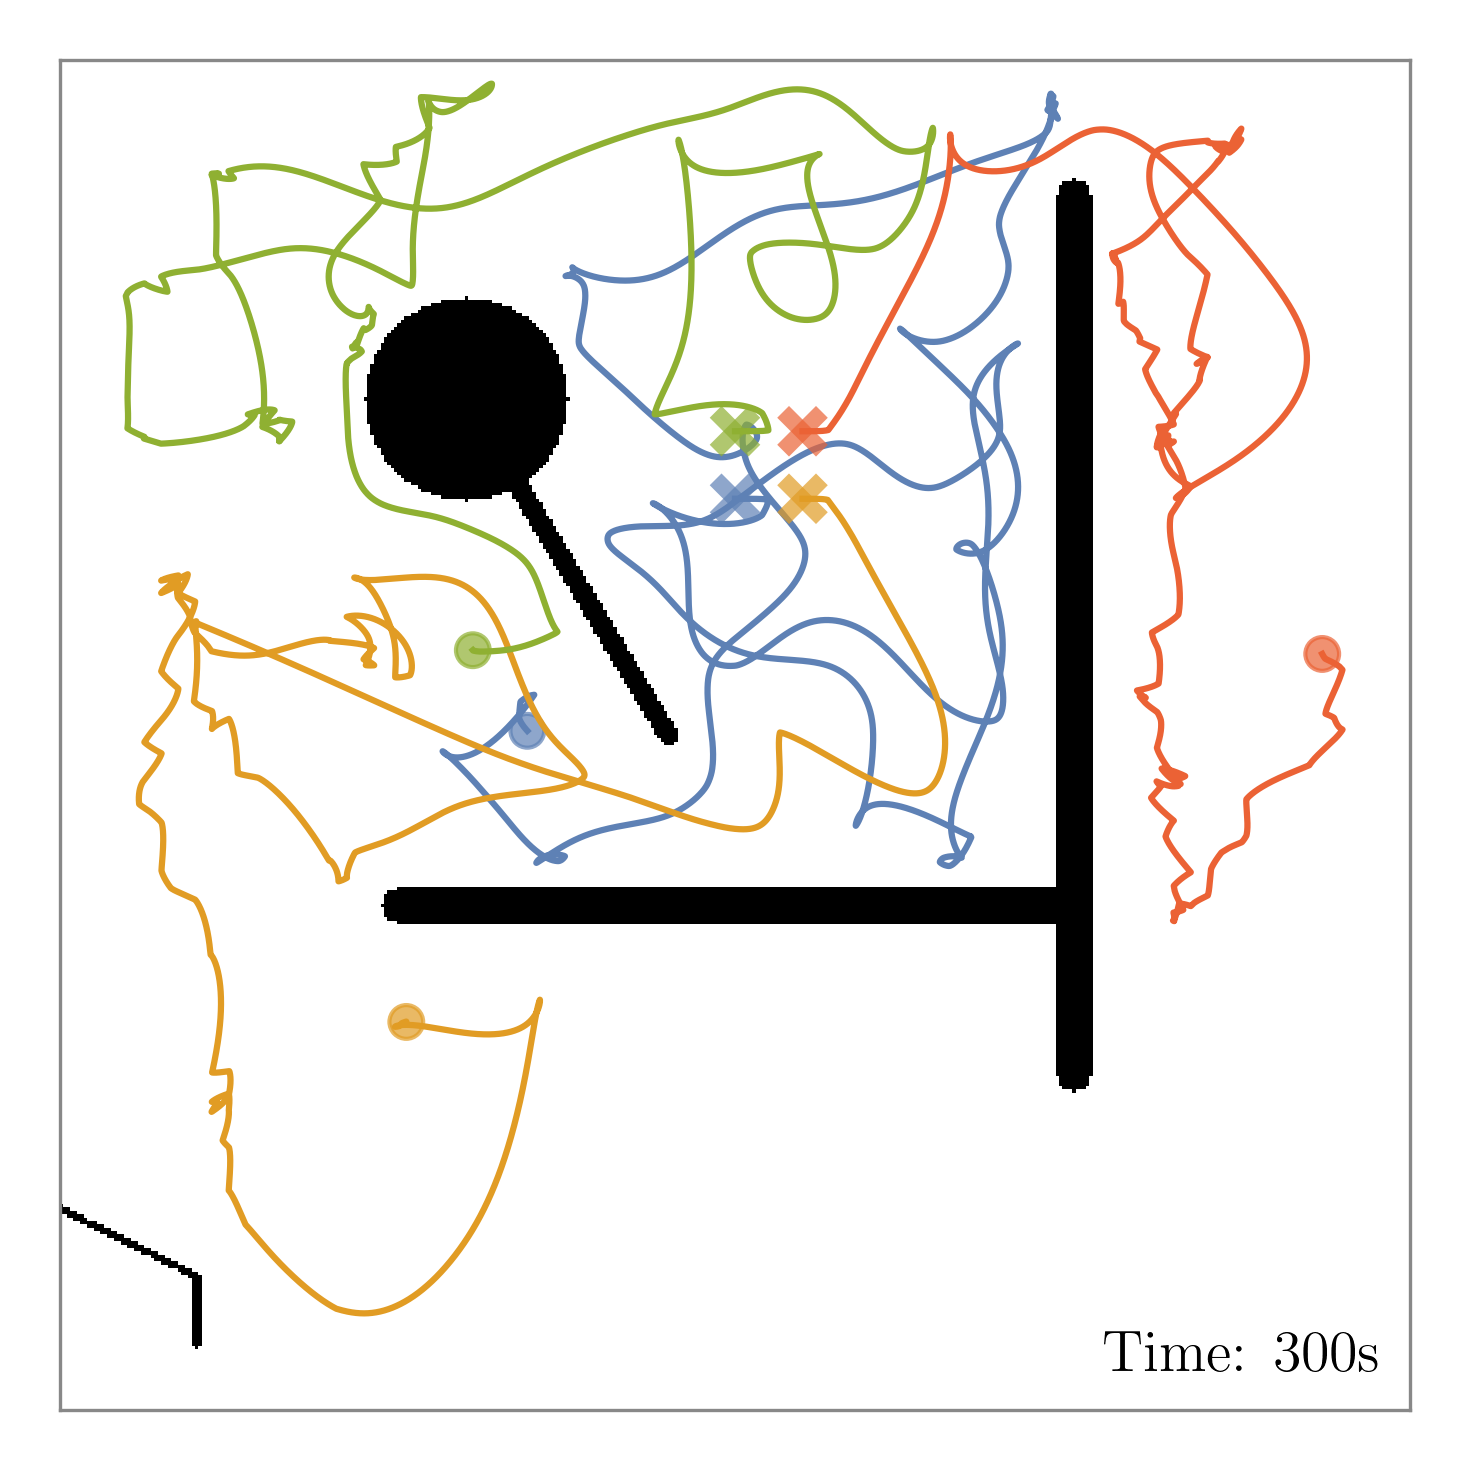
\includegraphics[width=\textwidth]{./figures/plots/gradient-paths/search:gradient-paths-(after-300s).png}
    \end{subfigure}
    \begin{subfigure}[b]{\w}
        \centering
        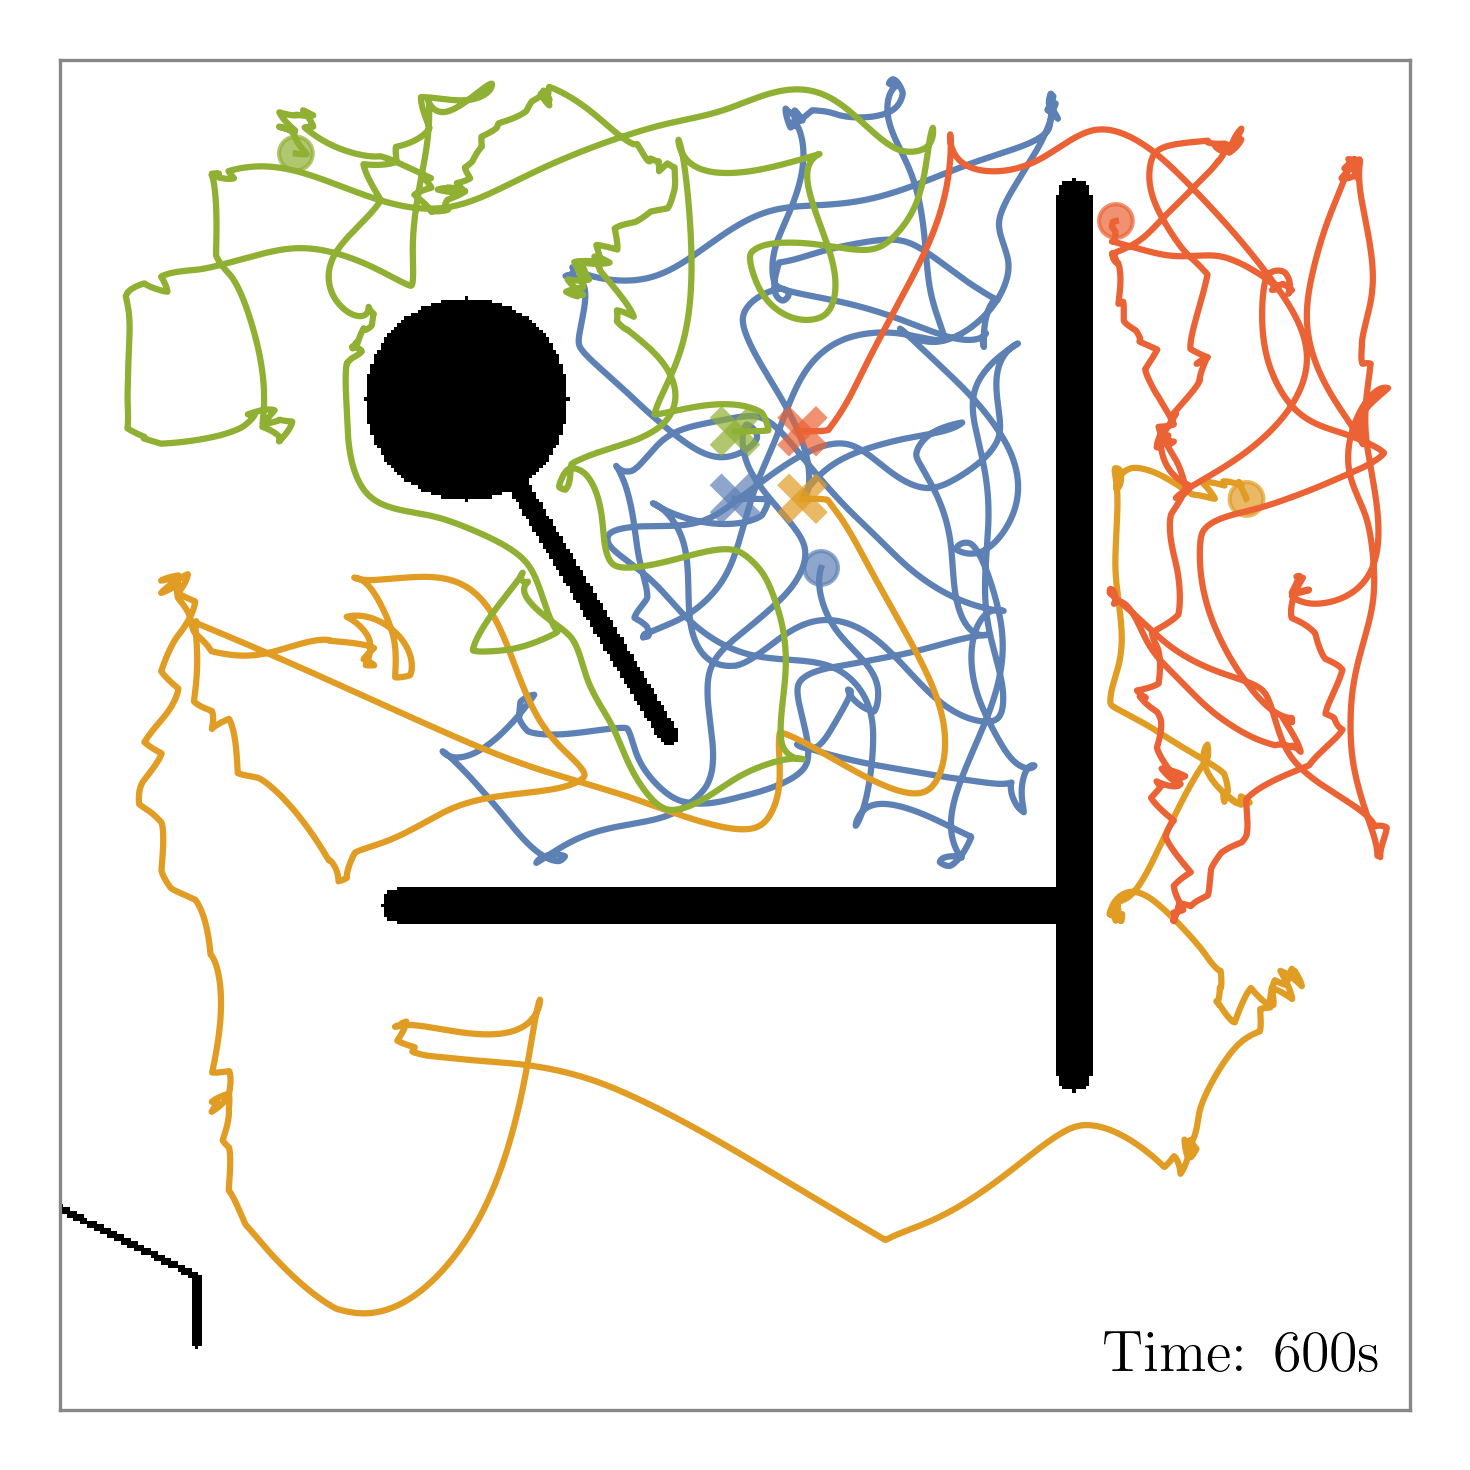
\includegraphics[width=\textwidth]{./figures/plots/gradient-paths/search:gradient-paths-(after-600s).png}
    \end{subfigure}
    \begin{subfigure}[b]{\w}
        \centering
        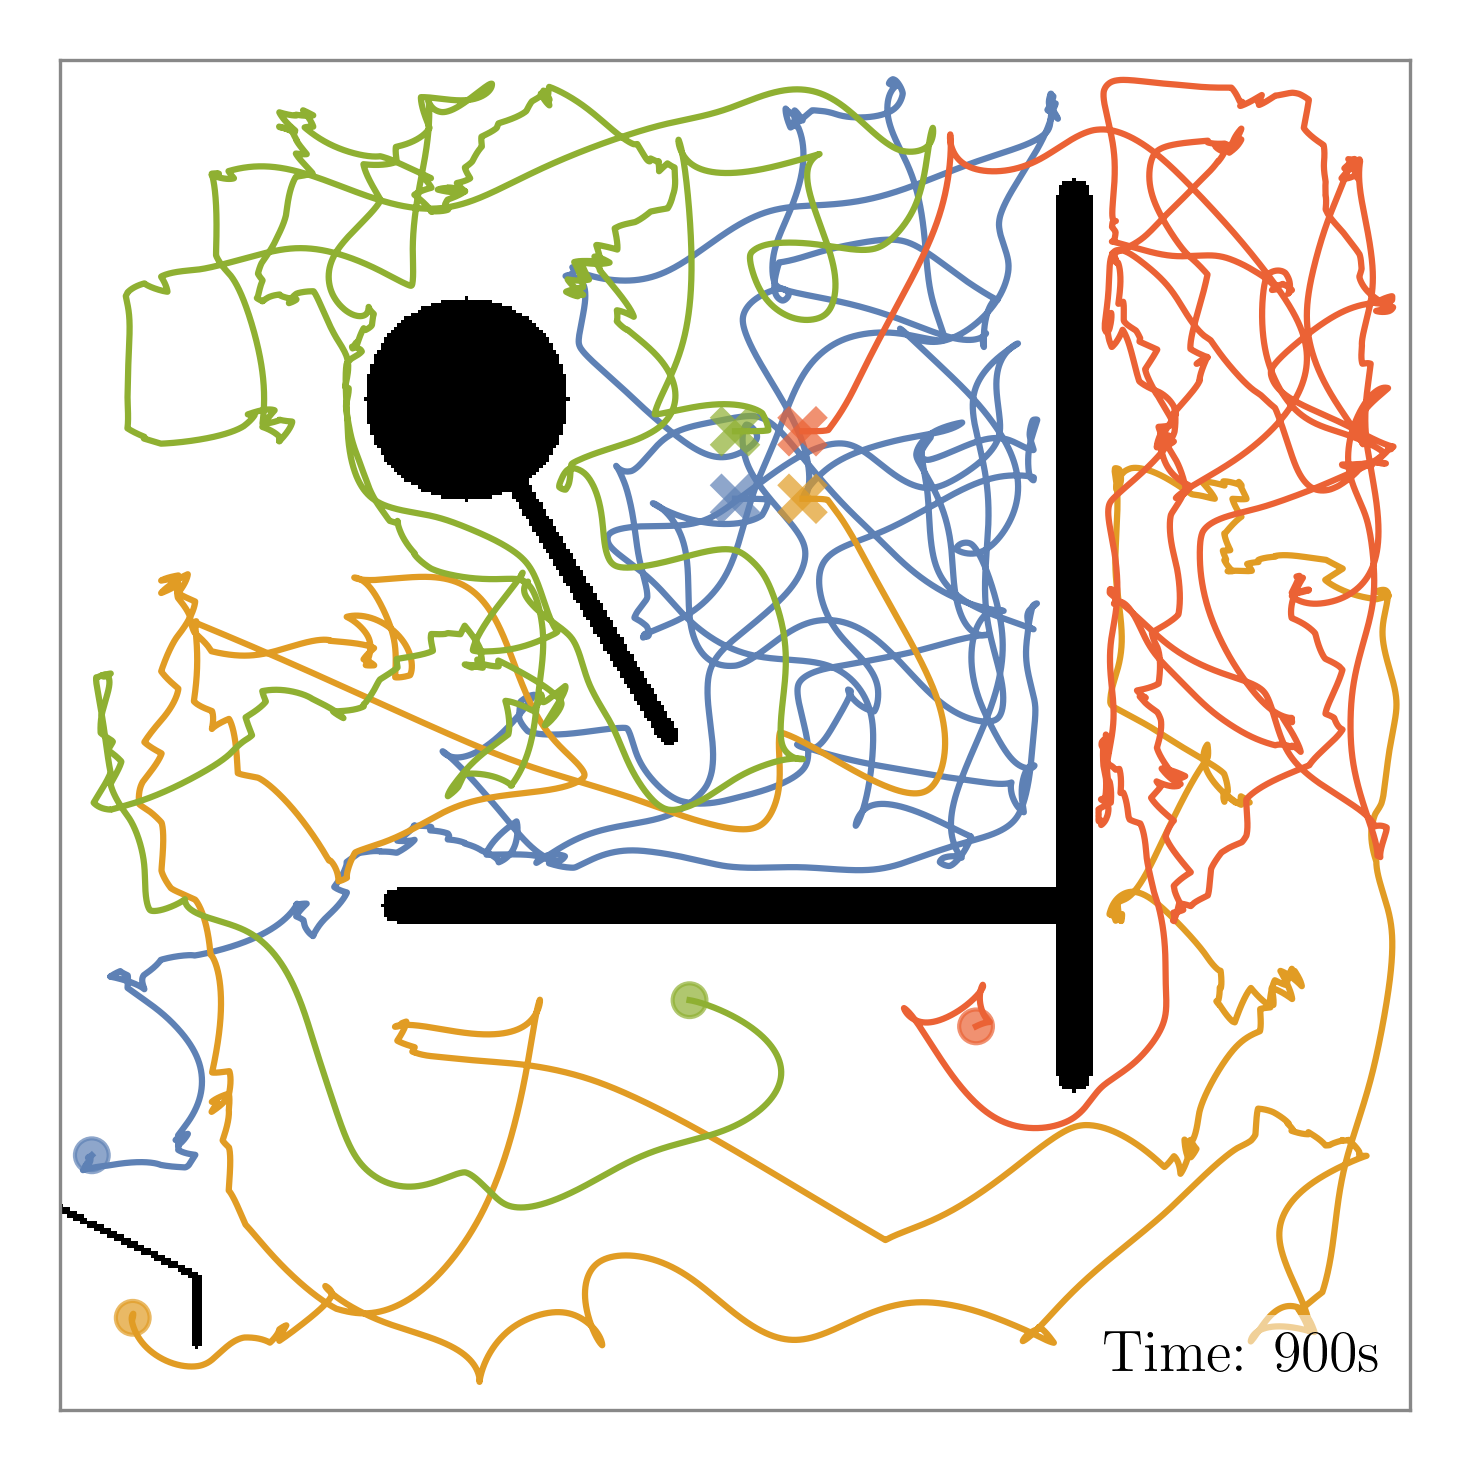
\includegraphics[width=\textwidth]{./figures/plots/gradient-paths/search:gradient-paths-(after-900s).png}
    \end{subfigure}
    \caption{Paths of 4 robots running the gradient based algorithm in an example world simulated using \texttt{simple\_sim}. Crosses mark robot starting positions and circles mark their end positions.}
    \label{fig:gradient-paths}
\end{figure}

The robots explore the map but tend to linger in areas that are already explored. 
This may be due to the limited range when calculating the gradient of the search grid. Robots also tend to linger when their search gradient becomes uncertain, which leads to more erratic paths. Generally, robots seem to switch between driving in smooth paths while exploring new area and in more jagged paths when lingering in already explored areas. To prevent this and promote map exploration, a mechanism to move them towards less explored areas of the map would be beneficial.

\subsection{Global Planner}

If the search gradient yields no clear direction, meaning the robot is unsure where to go, it can fall back on a more computationally expensive process to plan a path to a distant region.

In other scenarios, where computational resources are ample, the robot can rely entirely on path planning for navigation.

% TODO: Maybe make flowchart for this
The general procedure of the global planner is as follows:
\begin{enumerate}
  \item Generate a costmap (\cref{sec:costmap}).
  \item Identify frontiers and group them into regions (\cref{sec:frontier_exploration}).
  \item Evaluate the frontiers and select a goal (\cref{sec:frontier_exploration}).
  \item Plan a path using either a straight line or the A* algorithm (\cref{sec:path_planning}).
  \item Follow the path until the goal is reached or the path is invalidated (\cref{sec:path_following}).
\end{enumerate}

\subsubsection{Costmap}\label{sec:costmap}
To represent searched areas and obstacles, a costmap is constructed. 
The costmap has a resolution of $0.2\,\text{m}$ and is represented as a grid of cells. Each cell can be in one of three states:
\begin{itemize}
  \item \textbf{Searched:} Cells identified as covered in the search grid.
  \item \textbf{Unknown:} Cells not yet covered.
  \item \textbf{Obstacle:} Cells corresponding to static map obstacles or dynamic obstacles (e.g., other robots), inferred from the most recent LiDAR data.
\end{itemize}

% TODO: Show cost map and example of a planned route
\subsubsection{Frontier Exploration}\label{sec:frontier_exploration}
To determine a suitable goal, the robot performs frontier exploration.
A frontier is defined as a cell that separates searched and unknown areas.
Frontiers are detected using a Breadth-First Search starting from the robot’s current position, avoiding a full scan of the costmap and thereby reducing computation time.

Once frontiers are found, they are grouped into regions and evaluated based on three criteria:
\begin{itemize}
  \item Size of the frontier region.
  \item Distance to the robot.
  \item Required turn angle to face the frontier.
\end{itemize}
Additionally, a frontier must be sufficiently distant from any obstacle, as defined by a minimum clearance threshold.

\begin{figure}[H]
    \centering
    \begin{subfigure}[b]{0.45\textwidth}
        \centering
        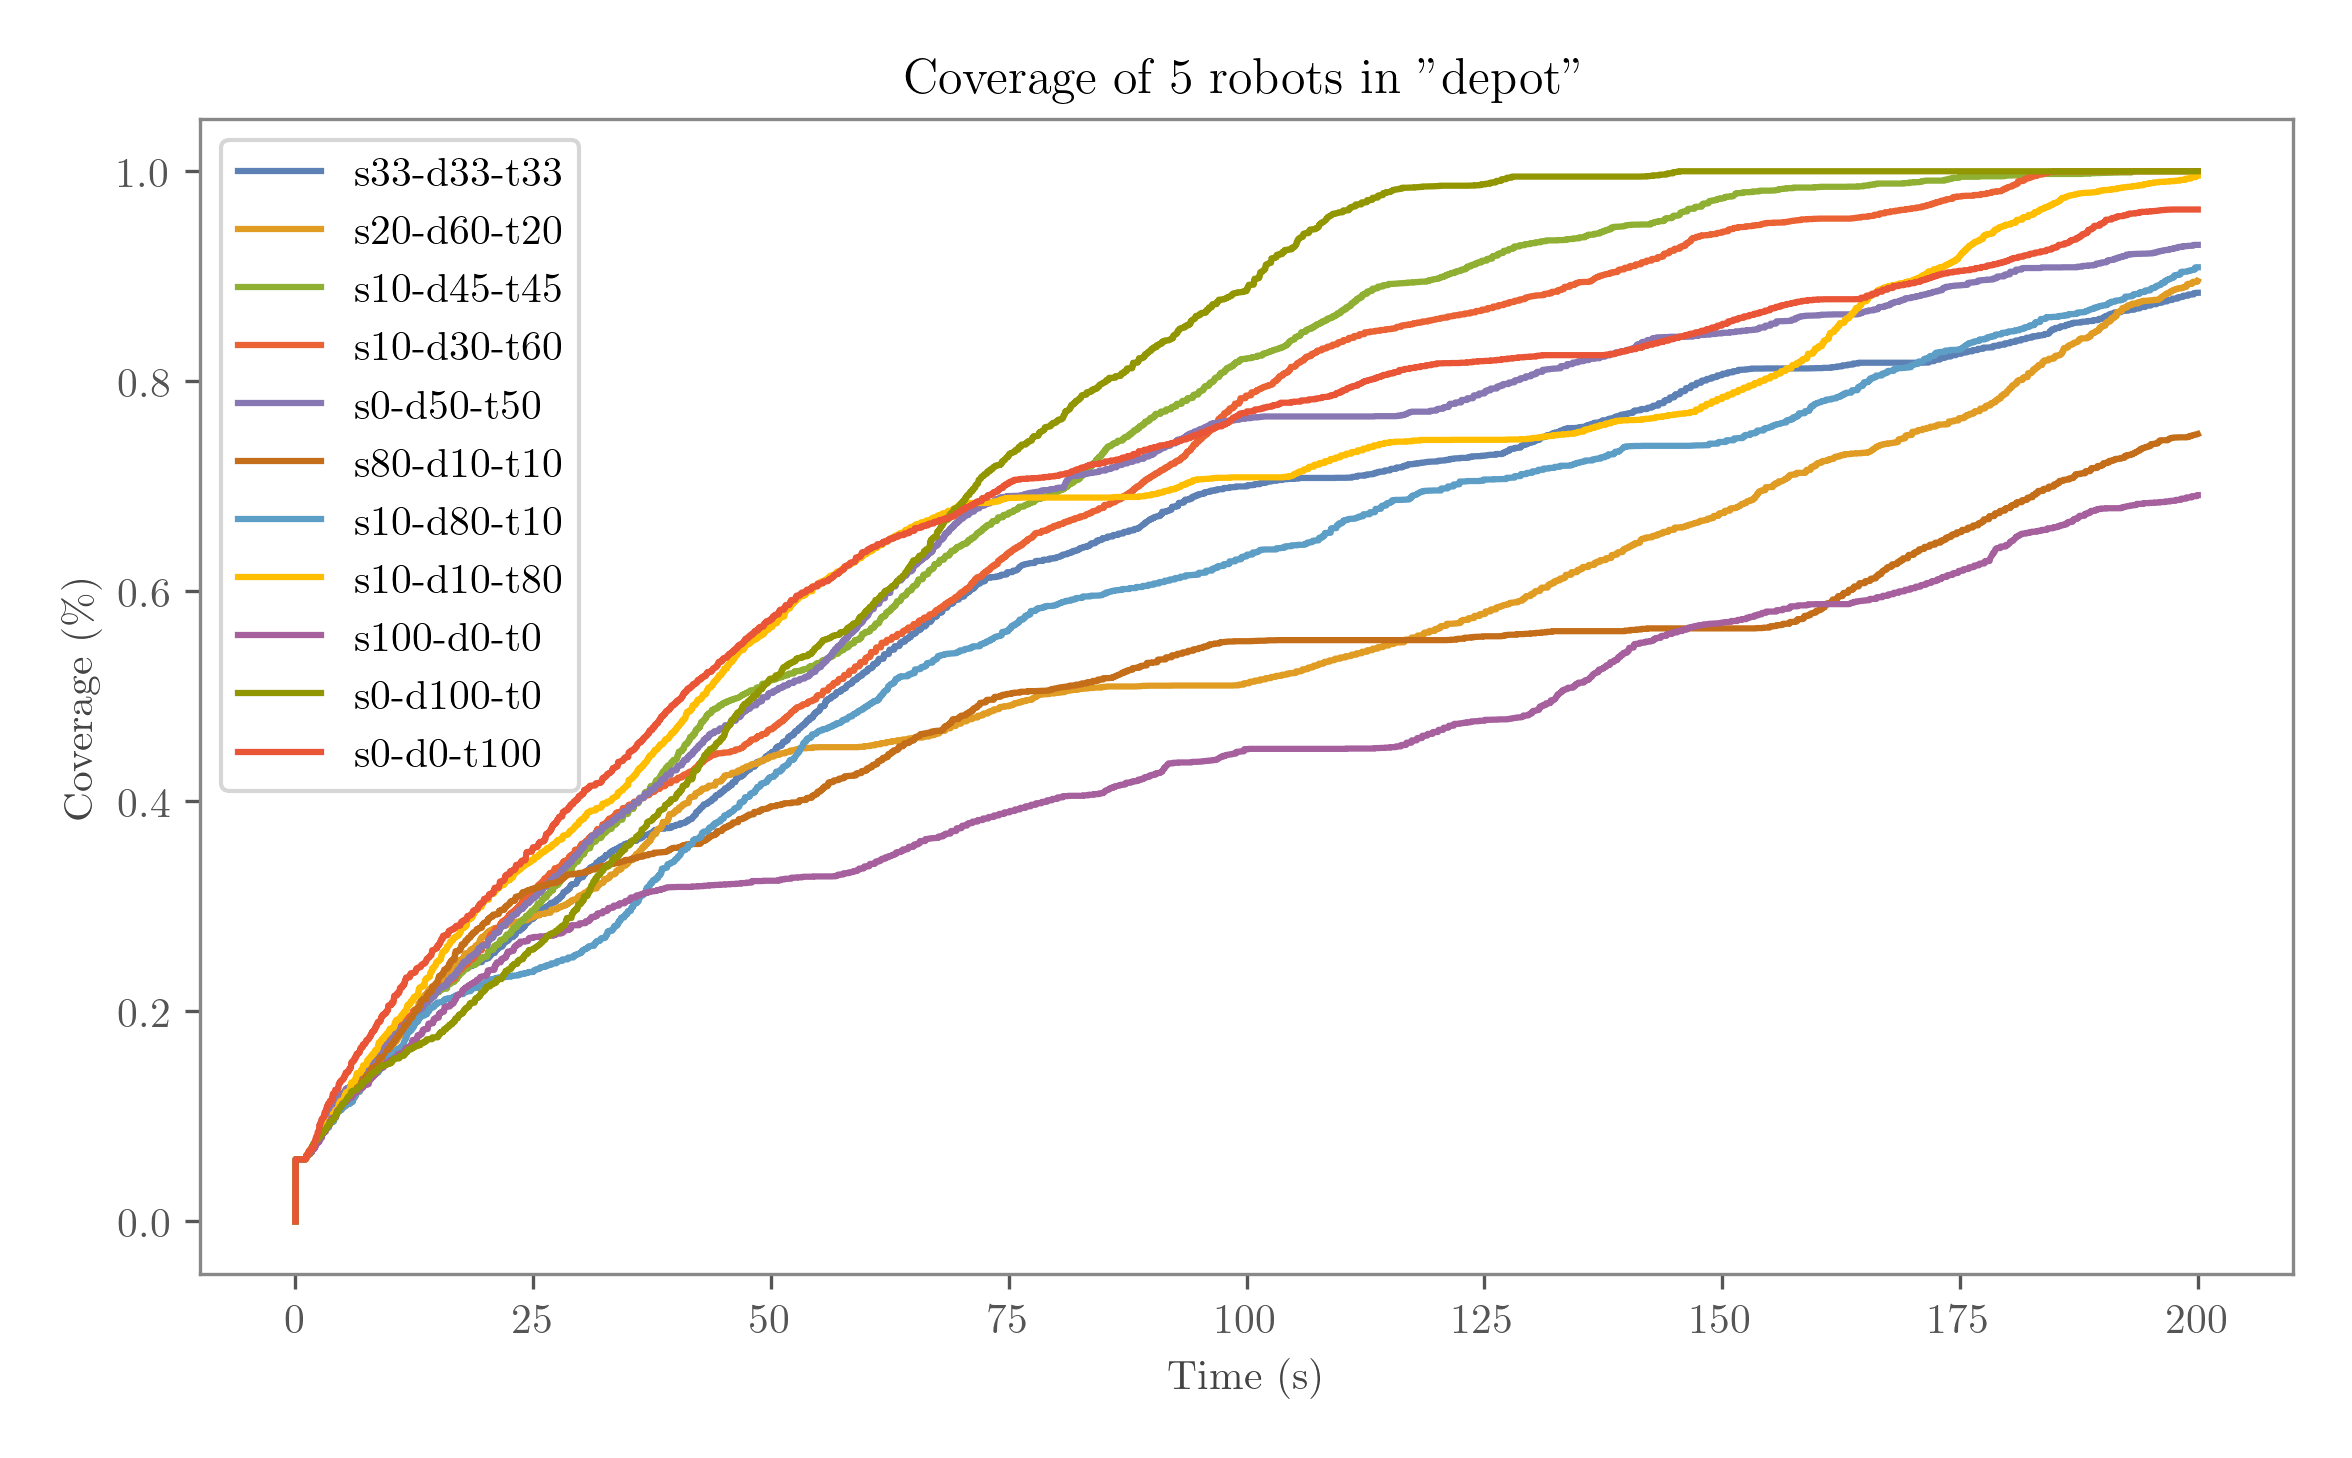
\includegraphics[width=\textwidth]{figures/frontier_eval_params_depot.png}
        \caption{Complex map}
    \end{subfigure}
    \begin{subfigure}[b]{0.45\textwidth}
        \centering
        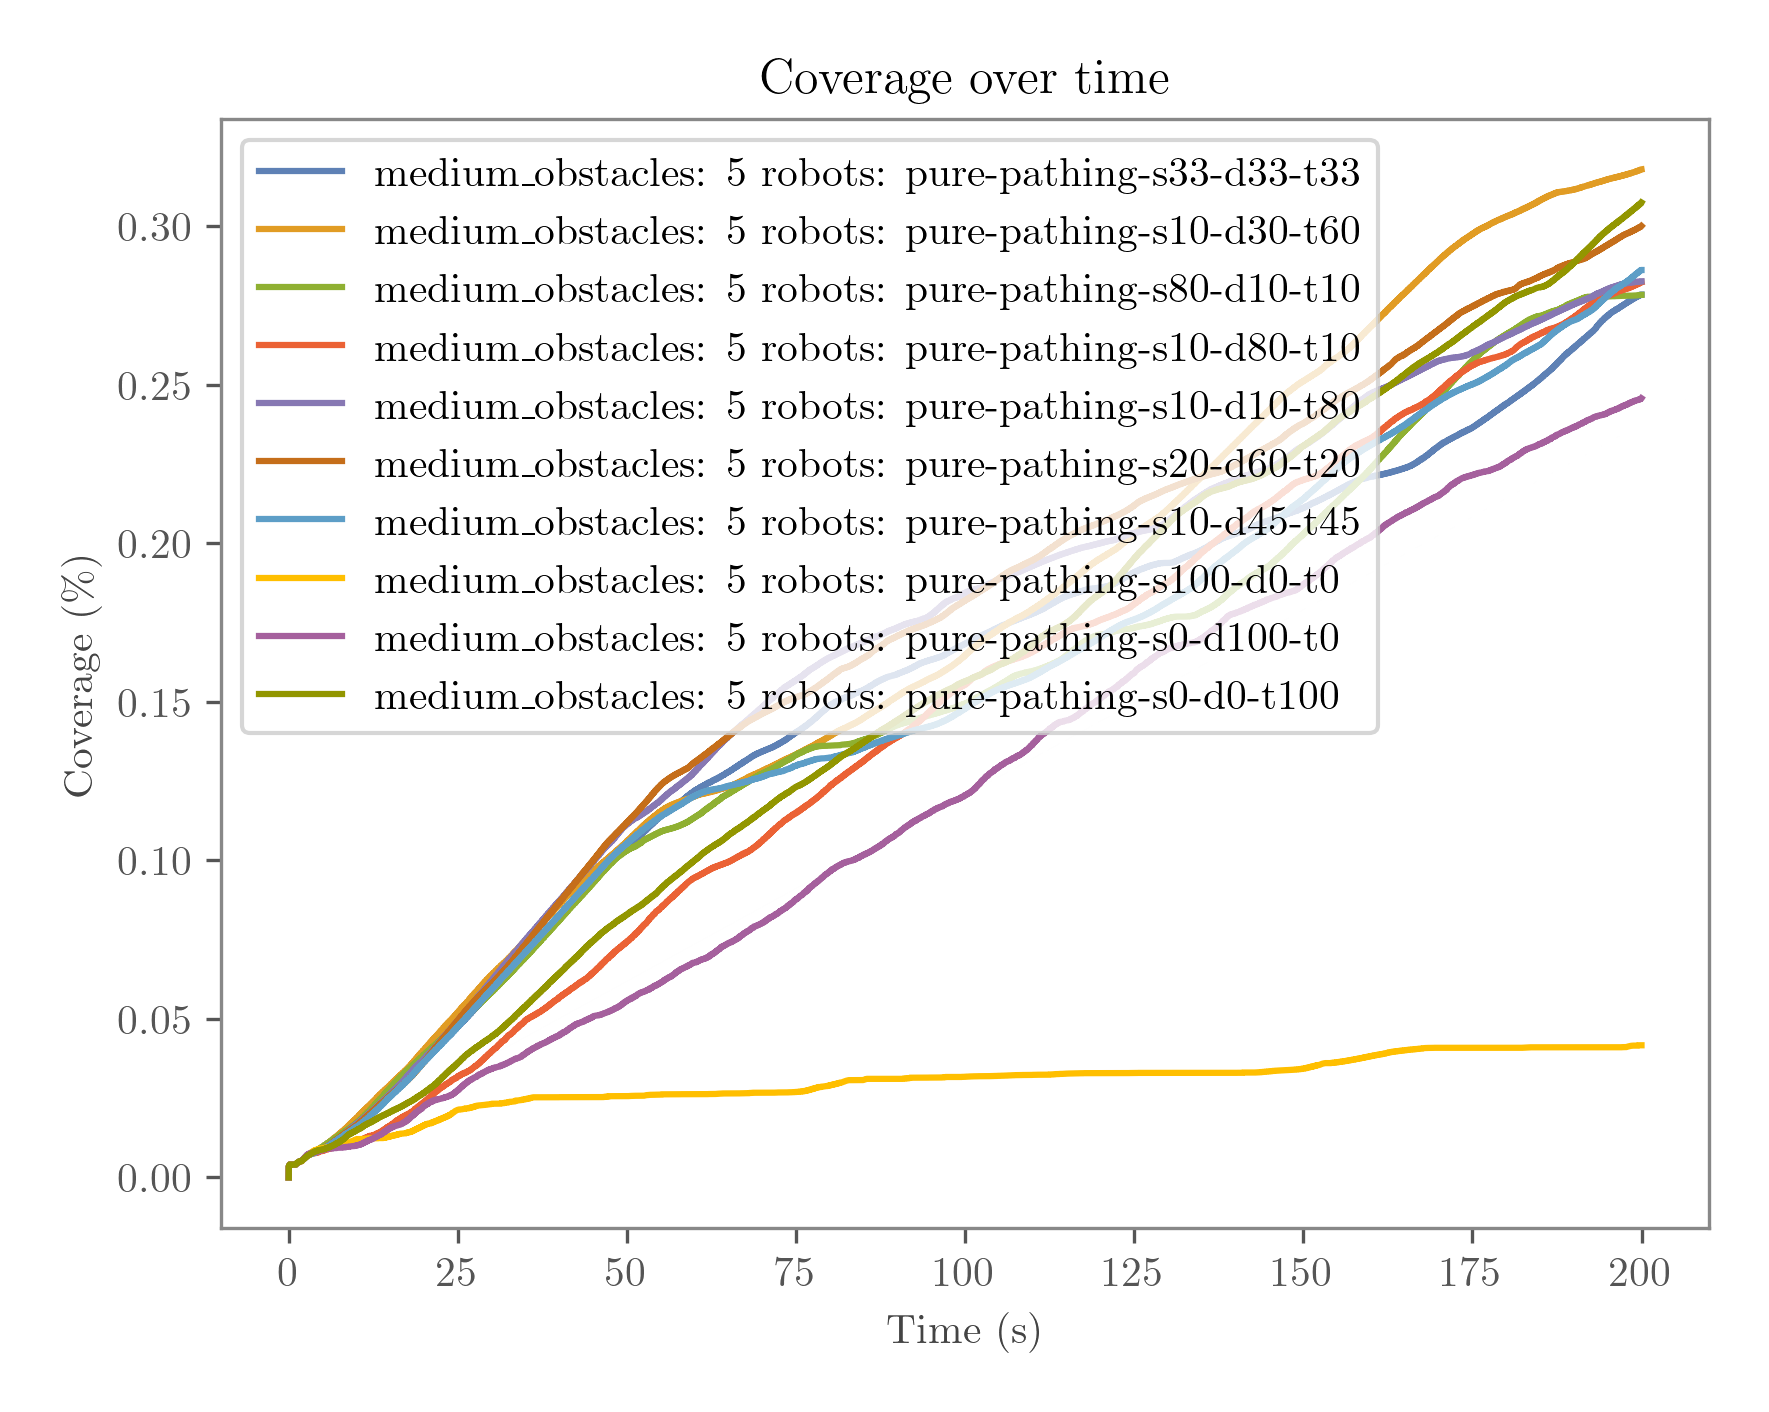
\includegraphics[width=\textwidth]{figures/frontier_eval_params_medium_obstacles.png}
        \caption{Simple map}
    \end{subfigure}
    \caption{Frontier evaluation parameters on two maps.}
    \label{fig:frontier-eval-params}
\end{figure}

These parameters were tested on two environments: a complex map with many narrow passages and a simpler one with fewer obstacles. Results for five robots are shown in \cref{fig:frontier-eval-params}. Each line label indicates the parameter weights: 
\texttt{sXX} for frontier size, \texttt{dXX} for distance, and \texttt{tXX} for turn angle.

All configurations were verified to eventually achieve full map coverage. Thus, only the speed of achieving this is used to evaluate performance.

As observed, configurations that favor high weights on distance and turn angle achieve faster coverage.
Turn angle is most significant, as turning reduces linear velocity, so robots prefer straight paths.
Distance weight encourages exploration of nearby frontiers first, promoting efficient local coverage.
Frontier size, on the other hand, had minimal impact. High weights on region size (e.g., \texttt{s100-d0-t0}) led to longer travel distances and frequent turning, reducing efficiency.

\subsubsection{Path Planning}\label{sec:path_planning}
After selecting a goal, a path is generated. First, a direct straight-line path is attempted. If it satisfies clearance requirements, it is used.
If not, the A* algorithm is employed to compute a valid path.

A* uses a heuristic based on both the cost so far and the estimated distance to the goal.
Cells are explored using a min-heap that prioritizes nodes with the lowest estimated total cost, enabling efficient search compared to Dijkstra’s algorithm, which evaluates all possible nodes.
Only positions that maintain a safe clearance from obstacles are included in the path.

\subsubsection{Path Following}\label{sec:path_following}
The planned path is a sequence of waypoints that the robot must follow to reach the goal.
As the robot approaches each subgoal within a defined threshold, the waypoint is marked as visited and removed from the list.

Even though the path is validated during planning, it is continuously re-evaluated in real time to account for dynamic obstacles, including other robots.
If validation fails, the robot still moves toward the next subgoal, but LiDAR-based obstacle avoidance is added to the target vector.
Should validation fail repeatedly, the robot attempts to replan the path. If replanning fails, a new goal is selected entirely.

As robots must maintain communication with others, if a robot becomes disconnected from the swarm, it will seek a new goal within the proximity grid to reestablish connectivity.
